Several experiments on this supervised learning challenge have been conducted using a variety of different techniques for classification are peformed on the two encoded datasets; FIN-Benthic and FIN-Benthic-concatenated. The classification methods are; k-Nearest Neighbors (kNN), Linear Discriminant Analysis (LDA), Support Vector Machines (SVM), Perceptron and Neural Networks (NN). Cross Validation (CV) are use for model selection to evaluate the best performing model. All the methods have been applied to the datasets on full dimensions and additionally with dimensionality reduction as a preprocessing step in the classification pipeline. Grid search have been used to search for good hyperparameters for all classifiers as well as dimensionality reduction techniques. Lastly existing Convolutional Neural Network architectures have been used on the raw images and using the promise of transfer learning to use a pretrained model to gain faster and better performing models on small datasets. For the transfer learning task the existing train, validation and test split have been used.

\paragraph{k-Nearest Neighbors (kNN)}

K-Nearest Neighbor is a distance-based classifier and as the name implies, classifies to the most common occuring class of the k-nearest neighbors. There exist a variety of distance metrics, some example are; euclidean, minikowski, manhanobli and manhattan distance. 

\begin{figure}[H]
    \centering
    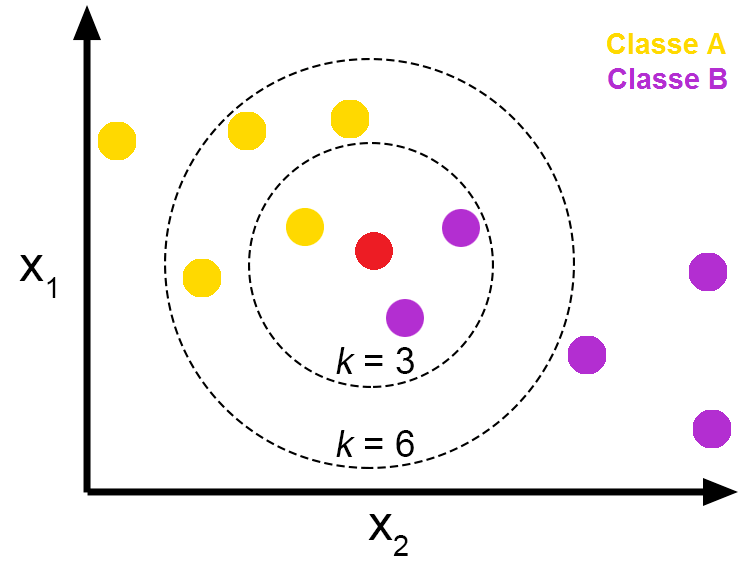
\includegraphics[width=0.4\textwidth]{figures/knn.png}
    \caption[]{k-Nearest Neighbor classifies the red sample to class B for $k=3$, however for $k=6$ it classifies to class A. Credits: Italo José}
    \label{fig:knn}
\end{figure}

\paragraph{Linear Discrmininat Analysis (LDA)}

Linear Discrmininat Analysis is a linear transformation of the data. The linear transformation is an optimization, that tries to maximize the distance between classes and minimize the distance within a class\todo{elaborate on decision boundary}. The classifier can also be used for dimensionality reduction, this would be further explained later.

\begin{figure}[H]
    \centering
    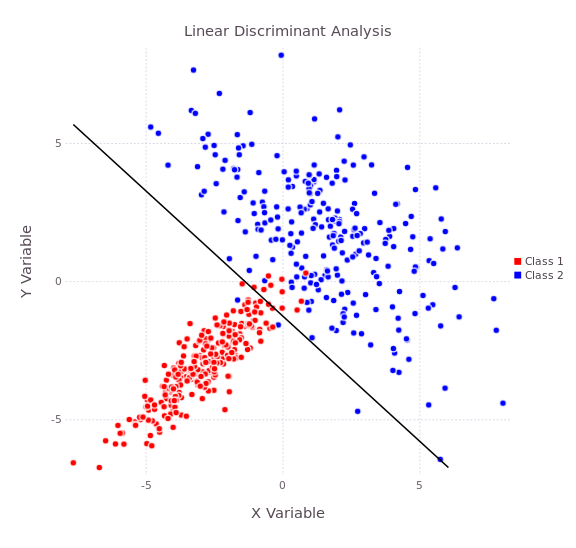
\includegraphics[width=0.4\textwidth]{figures/lda_deci.png}
    \caption[]{Credits: Tim Thatcher}
    \label{fig:lda_dec}
\end{figure}

\paragraph{Support Vector Machine (SVM)}

SVM can be used for classification. SVM tries to find the decision hyperplanes between the class and the rest of the data for \textit{"One-vs-Rest"} classification scheme using support vectors. 
The margin between the classes can either be a hard-marign or a soft-margin. A hard-margin essentially means only the support vectors on the edge of the margin are used to define the decision hyperplane. A soft-margin on the hands defines a hinge loss function.\todo{elaborate on hinge loss and margin. essetially just svm might need some reading}

SVM can be used on data which is not linearly seperable by applying the kernel trick. The kernel...  

\begin{figure}[H]
    \centering
    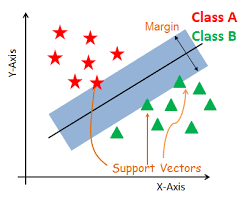
\includegraphics[width=0.4\textwidth]{figures/svm.png}
    \caption[]{Credits: Avinash Navlani}
    \label{fig:svm}
\end{figure}

\paragraph{Perceptron}

Perceptrons produces a linear decision function and only performs well on linearly seperable data. 

\begin{figure}[H]
    \centering
    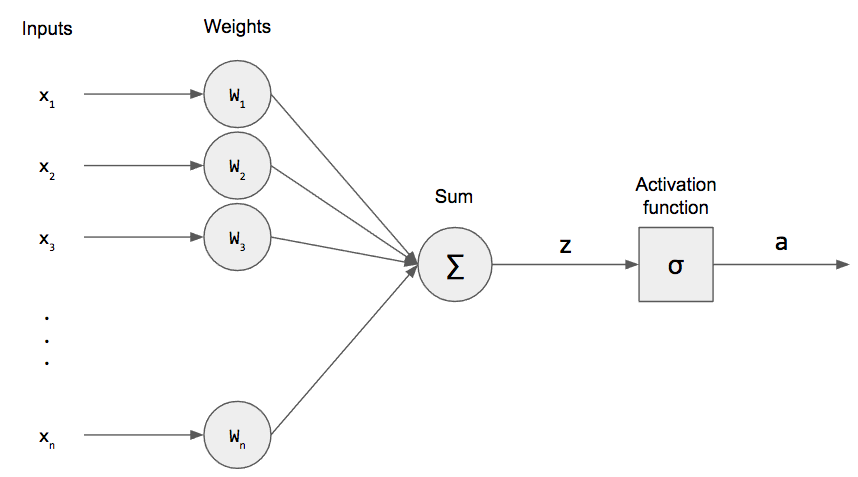
\includegraphics[width=0.4\textwidth]{figures/perceptron.png}
    \caption[]{The perceptron takes a feature vector as input. All the feature are multiplied by a weight. The weight are then summed to what is called a weighted sum. An activation function are applied to the weighted sum. The output of the activation function is the classification. Credits: Stanley Obumneme Dukor}
    \label{fig:perc}
\end{figure}

The perceptron are trained by iteratively updating the weights to produce the correct output for the training data. The loss function are rather simple, if the sample is correctly classified th loss function will output zero and it will output 1 if misclassified. This means the perceptron's weight are only updated when is fails to classify a sample. 

\paragraph{Neural Network (NN)}

Neural Networks extends the perceptron by adding a number of layers between the input and the output. These layers are referred to as hidden layers. The NN produces a non-linear decision function, thus overcomes the short comming of the perceptron.  

\begin{figure}[H]
    \centering
    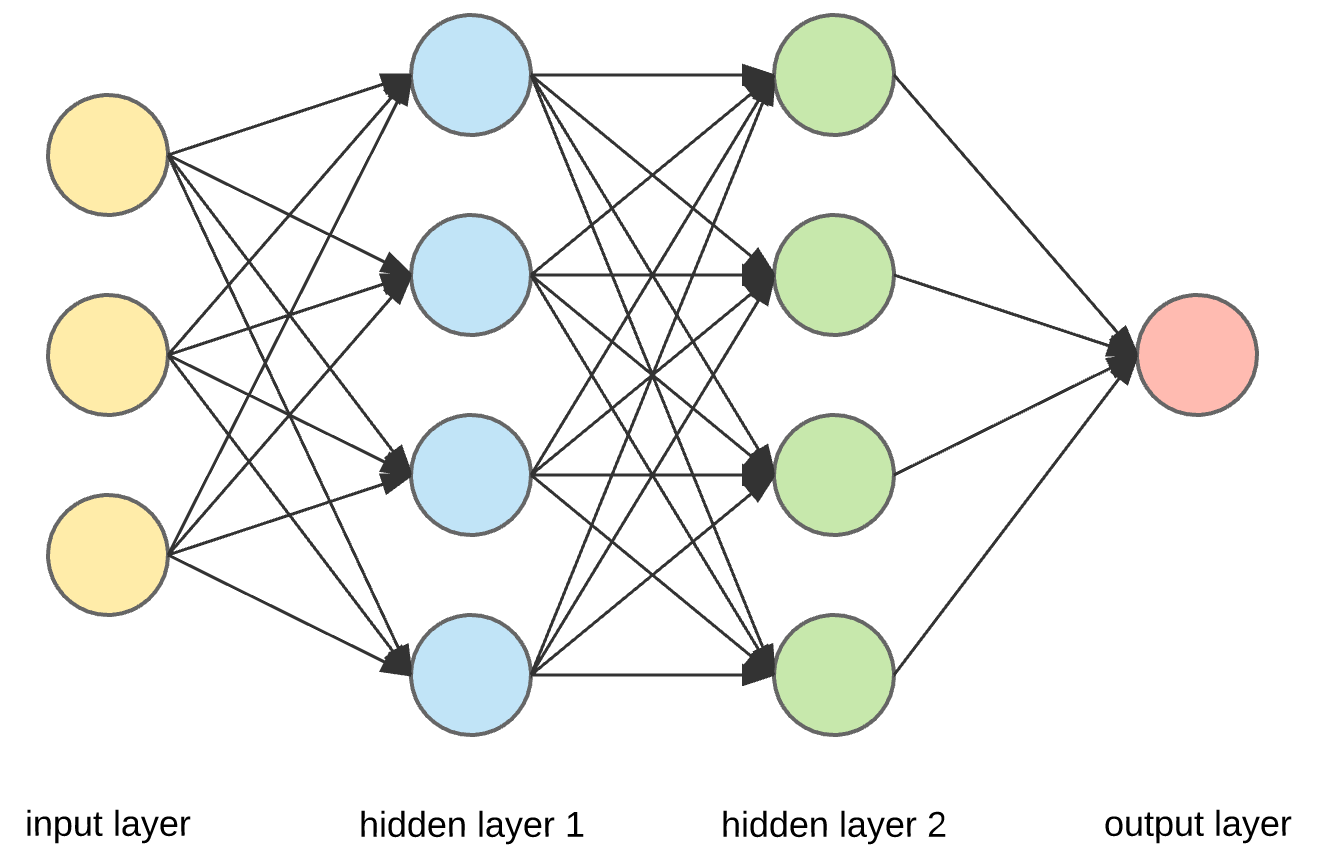
\includegraphics[width=0.4\textwidth]{figures/nn.png}
    \caption[]{Neural Network with two hidden layers and each layer is fomred by a number of neurons. A fully-connected dense neural network receives all output from previous layer as input. The input are multiplied by the neuron's weight and adding bias. At last the non-linear acitvation function is applied. Credits: Arden Dertat}
    \label{fig:nn}
\end{figure}

Training a NN is way more complex than a perceptron. The training are done using feedforward and back-propagation. Training vectors are given to the network, where all nodes do their operations upon receiving and ninput anf feeding it forward to the next layer, when it reaches the end of the network and error term is computed using the loss function. The error are then backpropagted. throuout the network, where the nodes' contribution to the error is computed. Using gradients the network weight are optimized. 

\paragraph{Convolutional Neural Network (CNN)}

\paragraph{Dimensionality Reduction}

Dimensionality reduction as the name implies downscales the feature space into a lower dimnesional space. The techniques used in this paper is the already covered LDA and Principal Component Analysis (PCA).

\subparagraph{Principal Component Analysis (PCA)}

PCA is a linear transformation onto a smaller feature space. The number of dimensions i.e. principal components are a hyperparameter. PCA is an unsupervised method, that tries to encapsulate as much as the variance as possible. The first component i.e. dimension is a projection a long the axis of the data with the variance, the second component is the axis with second most variance and so on, as the figure X shows.

\begin{figure}[H]
    \centering
    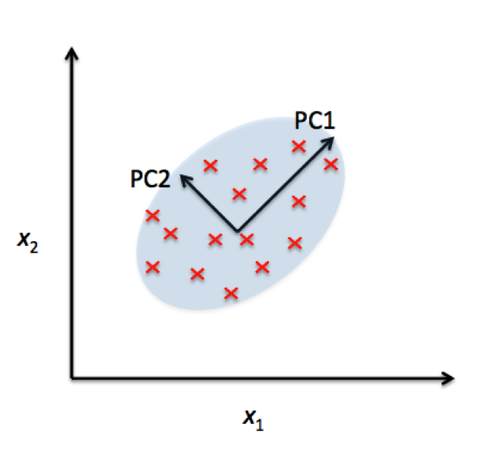
\includegraphics[width=0.4\textwidth]{figures/pca.png}
    \caption[]{Principal Component Analysis in a 2 dimensional space. PCA rotates the data to be perpendicular to the principal components axises. Credits: Sebastian Raschka}
    \label{fig:pca}
\end{figure}

\subparagraph{Linear Discriminant Analysis (LDA)}
As mention LDA can be used for dimensionality reduction as well. One must specify the $n$ number of components i.e. dimensions to transform the data onto, if the $n$ are less than the original data's dimensions D, the the number of dimensions will be reduced. 

\begin{figure}[H]
    \centering
    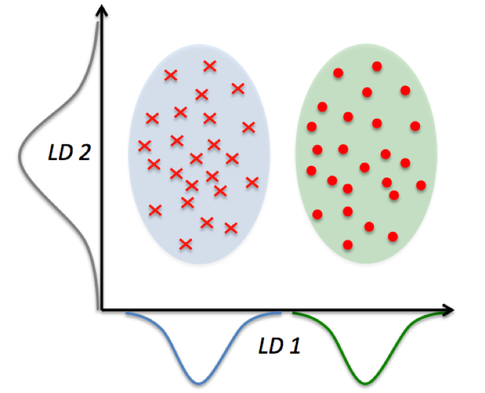
\includegraphics[width=0.4\textwidth]{figures/lda.png}
    \caption[]{Linear Discriminant Analysis project the data onto and axis, that maximize the distance between the classes and minimizes the distance within the respective classes. Credits: Sebastian Raschka}
    \label{fig:lda}
\end{figure}

\paragraph{Model Selection}

Model selection are procedures to train the best model and avoid overfitting the model to the training data. Overfitting is the pitfall of having a model, that desribes the training data too well, thus suffers to not generalising the true underlying structure of the data. Although other methods exists the two used in the paper are Validation Holdout and Cross Validation. 

\subparagraph{Validation Holdout}

Validation Holdout takes a fraction of your available labelled data and hold it out of the training procedure. 

\begin{figure}[H]
    \centering
    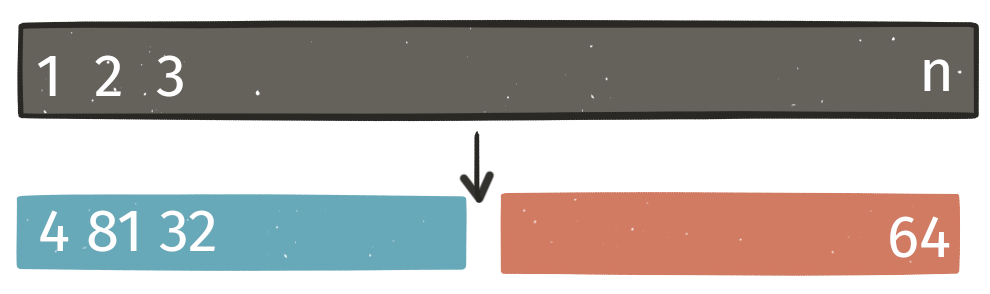
\includegraphics[width=0.4\textwidth]{figures/validationset.png}
    \caption[]{The validation subset is then used to validate the model's performance on data it has not been training.}
    \label{fig:val_holdout}
\end{figure}

The assumption is, that the holdout set resembles the true data, and if the model performs well on both training and validation it is assumed to be a good model. The split is typically made 70/30 for training data and validation data respectively. 

\subparagraph{Cross Validation (CV)}

Cross Validation extends on the holdout validation. $k$-fold Cross Validation create $k$ experiments compared to one. The entire data set are split in $k$ folds, for every $k$ step one subset is for validation and the remaining $k-1$ fold are used for training. Figure \ref{fig:cv} illustrates the idea. 

\begin{figure}[H]
    \centering
    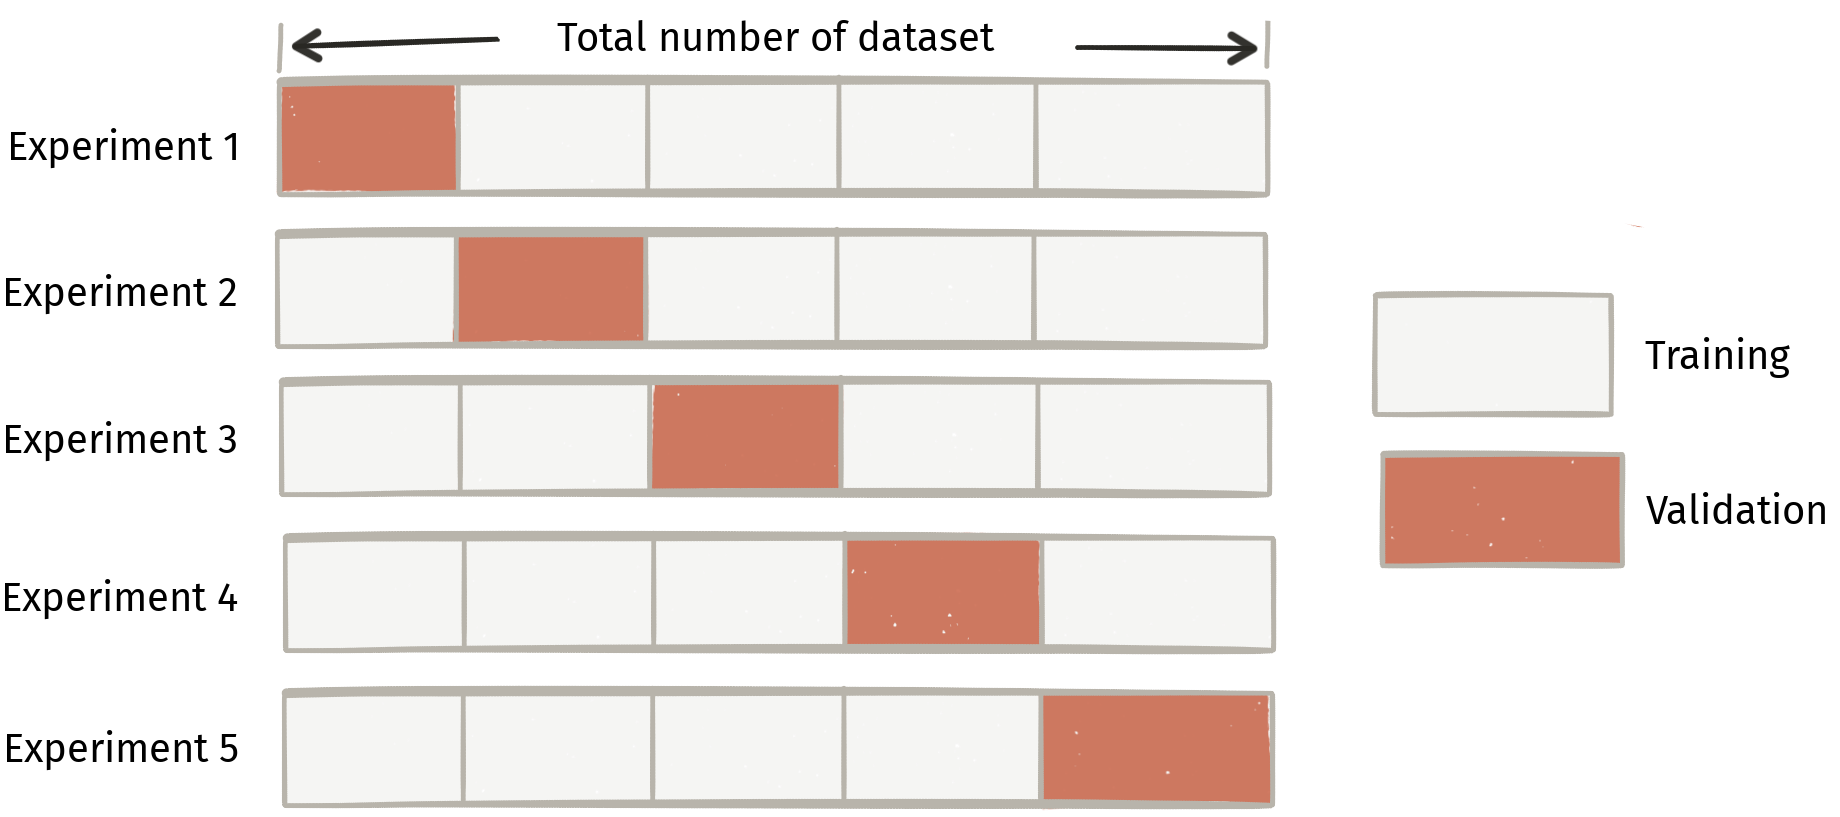
\includegraphics[width=0.5\textwidth]{figures/cv.png}
    \caption[]{Cross Validation ensures that the model have been trained on all the data and validated as well. The selection folds are typically either $k=5$ or $k=10$. }
    \label{fig:cv}
\end{figure}

\paragraph{Hyperparameter Search}

There are mainly two approaches to search for hyperparameters; Random Search and Grid Search other than heuristic guessing. In this paper Grid Search are used.

\subparagraph{Grid Search}

Grid Search is an approach to seek better hyperparameters for your model. You specify a set of options for all hyperparameters and then seacrh all possible combination in the grid. 

\begin{figure}[H]
    \centering
    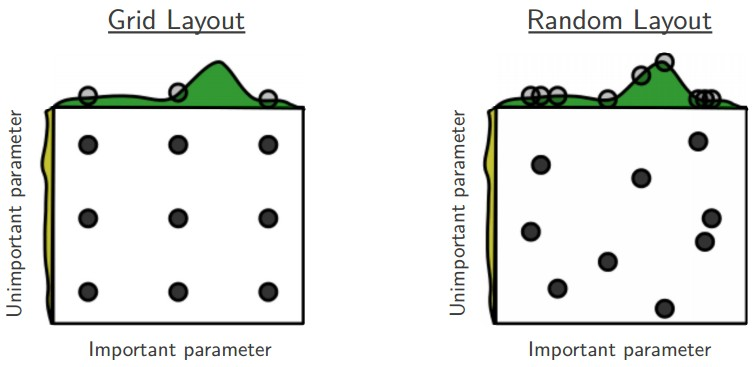
\includegraphics[width=0.4\textwidth]{figures/gridsearch_vs_randomsearch.jpeg}
    \caption[]{Grid search is a systematic approach to explore a broader space of hyperparameter although at the cost of additional time. The down-side of this approch is, that it is still based on intuition of good hyperparameters. The random approach are also widely used and might be preffered, as it may find a sweet spot, that goes beyond human intuition, however that is no guarantee and it is still time costly \cite{Bergstra}. Credits: Bergstra and Bengio}
    \label{fig:gs_vs_rs}
\end{figure}

  